% SPDX-License-Identifier: CC-BY-4.0
% DBOR specification - Dense Binary Object Representation
% Copyright (C) 2020 Daniel Lutz <dlu-ch@users.noreply.github.com>

\section{Introduction}
%%%%%%%%%%%%%%%%%%%%%%


\subsection{Usage examples}
%%%%%%%%%%%%%%%%%%%%%%%%%%%

\paragraph{Marshalling of a command (remote procedure call)}

Assume a distributed system of nodes, connected by slow serial point-to-point links (e.g. EIA-232 like).

The interface of a node is modelled as a hierarchical state machine, parametrized by typed parameters
(e.g. "desired flow rate in $\text{m}^3/\text{s}$") with non-negative integers as unique (per node) identifiers
and controlled by commands.

Each commands has a non-negative integer as a unique (per node) identifier and an associated sequence of
(typed) formal arguments.
For each command, the first argument is a dictionary of parameters (key: identifier, value: new value) to be
atomically set if the command succeeds and left untouched otherwise.
For example: \texttt{startPump(parametersToSetBefore, controlMode)} with identifier 12.

\medskip
\begin{BeginParPenalty}
    A specific call of this command with actual arguments can be described by a sequence of objects like this:
    \begin{quote}
        $42$, \{\}, $1$ or \\
        $42$, \{$3$: $0.010$, $9$: $0$, $11$: $\infty$\}, $2$.
    \end{quote}
\end{BeginParPenalty}

\begin{BeginParPenalty}
    When DBOR-encoded, this becomes:
    \begin{quote}
        \ByteSequence{
            \DborFirstByteHex{Number}{0C},
            \DborFirstByteHex{Dictionary}{A0},
            \DborFirstByteHex{Number}{01}
        }
        or \\
        \ByteSequence{
            \DborFirstByteHex{Number}{0C},
            \DborFirstByteHex{Dictionary}{A7}, % {
                \DborFirstByteHex{Number}{03},
                \DborFirstByteHex{Number}{E9}, \DborNextByteHex{01},
                %
                \DborFirstByteHex{Number}{09},
                \DborFirstByteHex{Number}{00},
                %
                \DborFirstByteHex{Number}{0B},
                \DborFirstByteHex{Numberlike}{FE},
            \DborFirstByteHex{Number}{02}
        }, respectively.
    \end{quote}
\end{BeginParPenalty}

\paragraph{Representation of a run-time event}

Run-time errors and similar events may be detected in every conceivable context -
e.g. in an interrupt handler where no dynamic memory can be allocated.
Instead of just discarding all dynamic information, one can proceed as follows to make the most of the available
(pre-allocated) memory:

\begin{enumerate}
    \item
    Choose an integer $n_{\text{max}} \le 3$, e.g. $n_{\text{max}} = 16$ and provide a means to successfully store at
    least \emph{one} object of size $\le n_{\text{max}}$ at any time, for example in a look-free queue.

    \item
    Assign each run-time event type a unique integer identifier like this:
    \begin{itemize}
        \item an even value > 0 if the event is application-related
        \item an odd value > 0 if the event is developer-related
        \item an even value < 0 if the event is a fatal error
        \item an odd value < 0 if the event is a non-fatal error
    \end{itemize}
    When DBOR-encoded, the identifier must be at most $n_{\text{max}} - 2$ bytes long.

    Associate each such run-time event type with a sequence of context objects describing the cause or detection context
    (e.g. measured current), ordered by preciousness of the information (most precious first), such that the meaning
    of no context objects does depend on other context objects later in the sequence.

    \item
    Whenever the event occurs:
    Build a DBOR-encoded event object of size $\ne n_{\text{max}}$, consisting the
    identifier of the event type, followed by the sequence of all context objects, only so much of its last objects
    omitted that the resulting size is $\ne n_{\text{max}}$.%
    \footnote{%
        When $n_{\text{max}} \le 25$, the \DborIntegerToken{} of the contained \DborSequenceValue{}
        is exactly 1~byte long which makes encoding especially fast and simple.
    }
    Then store it.
\end{enumerate}

\begin{BeginParPenalty}
    Such an event may look like this:
    \begin{quote}
        $-7$, [$12 \cdot 2^{-3}$, $4$, "dlu-ch"].
    \end{quote}
\end{BeginParPenalty}

\begin{BeginParPenalty}
    When DBOR-encoded, this becomes:
    \begin{quote}
        % https://dlu-ch.github.io/dbor-js/encoder.html?q=-7%2C%20%5B12*2%5E-3%20%2C%204%2C%20%22dlu-ch%22%5D
        \ByteSequence{
            \DborFirstByteHex{Number}{26},
            \DborFirstByteHex{Sequence}{8A}, % [
                \DborFirstByteHex{Number}{C8}, \DborNextByteHex{38},
                \DborFirstByteHex{Number}{04},
                \DborFirstByteHex{String}{66},
                    \DborNextByteHex{64}, \DborNextByteHex{6C}, \DborNextByteHex{75}, \DborNextByteHex{2D},
                    \DborNextByteHex{63}, \DborNextByteHex{68}
        }.
    \end{quote}
\end{BeginParPenalty}

\paragraph{QR code in error dialog}

It may be beneficial to embed machine-readable detailed context information in
an error message whose text message has to be short and easy to understand.

\begin{BeginParPenalty}
    Think of this piece of information:
    \begin{quote}
        \newcommand{\h}{\hspace*{\leftmargin}}
        \{ \\
            \h "sys": \{ \\
                \h\h "artno": $987$, \\
                \h\h "sn": $123$, \\
                \h\h "v": "1.2.3" \\
            \h \}, \\
            \h "err": [ \\
                \h\h $-7$, [$12 \cdot 2^{-3}$, $4$, "dlu-ch"] \\
            \h ] \\
        \}
    \end{quote}
\end{BeginParPenalty}

\begin{BeginParPenalty}
    When DBOR-encoded, it becomes (without the $\HexNumber{\ldots}$):
    \begin{quote}
        % https://dlu-ch.github.io/dbor-js/encoder.html?q=%7B%0A%20%20%20%20%22sys%22%3A%20%7B%0A%20%20%20%20%20%20%20%20%22artno%22%3A%20987%2C%0A%20%20%20%20%20%20%20%20%22sn%22%3A%20123%2C%0A%20%20%20%20%20%20%20%20%22v%22%3A%20%221.2.3%22%0A%20%20%20%20%7D%2C%0A%20%20%20%20%22err%22%3A%20%5B%0A%20%20%20%20%20%20%20%20-7%2C%20%5B12*2%5E-3%20%2C%204%2C%20%22dlu-ch%22%5D%0A%20%20%20%20%5D%0A%7D

        \newcommand{\F}[2]{\DborFirstByte{#1}{#2}\Number}
        \newcommand{\N}[1]{\DborNextByte{#1}\Number}

        \newcolumntype{L}{>{}c<\ByteSep@{}}% package 'array'
        \newcommand{\ByteSep}{, }
        \begin{tabular}{@{} *{16}L}
            \hbox to 0pt{\hss$\ByteSequenceOpening$ }%
            \F{Dictionary}{B8}& \N{14}&  % {
                \F{String}{63}& \N{65}& \N{72}& \N{72}&
                \F{Sequence}{8C}&  % [
                    \F{Number}{26}&
                    \F{Sequence}{8A}&  % [
                        \F{Number}{C8}& \N{38}&
                        \F{Number}{04}&
                        \F{String}{66}&
                            \N{64}& \N{6C}& \N{75} \\ \N{2D}&
                            \N{63}& \N{68}&
                %
                \F{String}{63}& \N{73}& \N{79}& \N{73}&
                \F{Dictionary}{B6}&  % {
                    \F{String}{61}& \N{76}&
                    \F{String}{65}&
                        \N{31}& \N{2E}& \N{32}& \N{2E}&
                        \N{33} \\
                    %
                    \F{String}{62}& \N{73}& \N{6E}&
                    \F{Number}{18}& \N{63}&
                    %
                    \F{String}{65}&
                        \N{61}& \N{72}& \N{74}& \N{6E}&
                        \N{6F}&
                    \F{Number}{19}& \N{C3}& \N{02}
                    \let\ByteSep\relax \hbox to 0pt{$\ByteSequenceClosing$\hss}
        \end{tabular}
    \end{quote}
\end{BeginParPenalty}

The smallest corresponding \href{https://www.qrcode.com/en/about/version.html}{QR Code Model 2}
(ISO/IEC~18004:2015, 8-bit byte mode) is version~3 which has the size of $29 \times 29$~modules (pixels).%
\footnote{%
    Generated with
    \href{https://github.com/fukuchi/libqrencode/blob/v4.0.2/qrenc.c}{%
        \texttt{qrencode --8bit --size 1 --margin 0 --level L}}.
}

\begin{figure}[H]
    \begin{quote}
        \noindent
        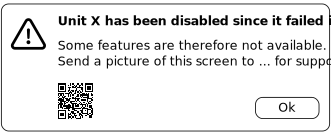
\includegraphics[scale=0.8]{example_error_dialog}%
        \caption{Error dialog with machine-readable context information.}
        \label{fig:class:Value}
    \end{quote}
\end{figure}


\subsection{Terms and notation}
%%%%%%%%%%%%%%%%%%%%%%%%%%%%%%%

In this specification, $N$ always denotes the constant
$\sum_{i = 1}^8 2^{8i}
= 18\,519\,084\,246\,547\,628\,288
\approx 1.003922 \cdot 2^{64}$.

\noindent
{%
    \setlength\extrarowheight{0.8ex}%
    \begin{tabular}{@{} p{.1\textwidth} p{.8\textwidth}}
        $\SetOfReals$: &
            the set of real numbers \\
        $\SetOfIntegers$: &
            the set of integers $\subset \SetOfReals$ \\
        $\IntegerInterval{a}{b}$: &
            $\{i \in \SetOfIntegers\colon a \le i \le b\}$ \\
        $\ByteSequence{a, b, \ldots}$: &
            byte sequence, starting with byte $a$ \\
        $a \Concat b$: &
            concatenation of bytes sequences $a$, $b$: $a$ followed by $b$ \\
        $\|a\|$: &
            size of bytes sequence $a$ in byte \\
        "\dots": &
            UTF-8 encoded Unicode string in Normalization Form C (NFC) \\
    \end{tabular}%
}
